Trataremos de aprovechar el hecho de que la colección está ordenada y vamos a hacer algo distinto: nuestro espacio de búsqueda se irá achicando a segmentos cada vez menores de la colección original. La idea es descartar segmentos de la lista donde el valor seguro que no puede estar:

\begin{enumerate}
	\item Consideramos como segmento inicial de búsqueda a la lista completa.
	\item Analizamos el punto medio del segmento (el valor central), si es el valor buscado, devolvemos el índice del punto medio.
	\item Si el valor central es mayor al buscado, podemos descartar el segmento que está desde el punto medio hacia la a derecha.
	\item Si el valor central es menor al buscado, podemos descartar el segmento que está desde el punto medio hacia la izquierda.
	\item Una vez descartado el segmento que no nos interesa, volvemos a analizar el segmento restante, de la misma forma.
	\item Si en algún momento el segmento a analizar tiene longitud 0 o negativa significa que el valor buscado no se encuentra en la coleción.
\end{enumerate}

Este algoritmo es un gran ejemplo de una estrategia de dividir y conquistar. Dividir y conquistar 
significa que dividimos el problema en partes más pequeñas, resolvemos dichas partes más pequeñas de 
alguna manera y luego reensamblamos todo el problema para obtener el resultado. Cuando realizamos una 
búsqueda binaria en una colección, primero verificamos el ítem central. Si el ítem que estamos 
buscando es menor que el ítem central, podemos simplemente realizar una búsqueda binaria en la mitad 
izquierda de la colección original. Del mismo modo, si el ítem es mayor, podemos realizar una 
búsqueda binaria en la mitad derecha. 

Para señalar la porción del segmento que se está analizando a cada paso, utilizaremos dos variables (izq y der) que contienen la posición de inicio y la posición de fin del segmento que se está considerando. De la misma manera usaremos la varible medio para contener la posición del punto medio del segmento.

En el gráfico que se incluye a continuación, vemos qué pasa cuando se busca el valor 18 en la lista [1, 3, 5, 7, 9, 11, 13, 15, 17, 19, 21, 23].

% TODO: \usepackage{graphicx} required
\begin{figure}[h!]
	\centering
	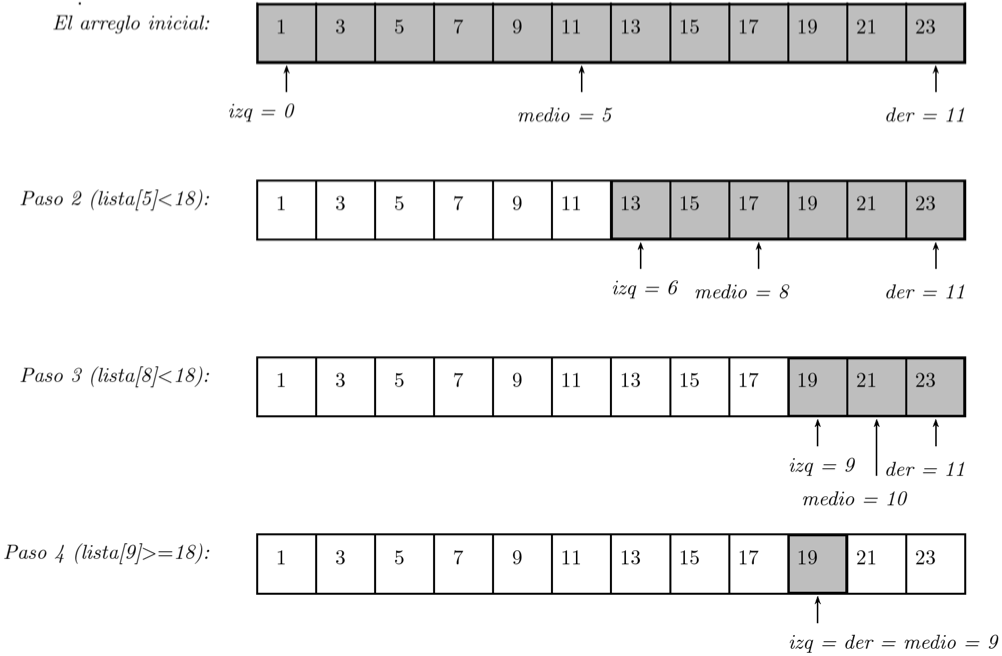
\includegraphics[width=0.7\linewidth]{img/f0801}


\end{figure}

